\section{Historia}

El término {\GAM} fue acuñado cerca del año 2008\cite{DefineGamefication}.
El objetivo fue crear un término que agrupara todas las ideas y elementos
utilizados en el diseño de juegos que pudiesen ser utilizados en otros contextos
(distintos a los de entretención).
En el año 2010, este término llega a ser conocido mundialmente  y esto se ve reflejado
 al aparecer como uno de los terminos mas buscados en google\cite{GamWorks}.

%\begin{figure}[!htb]
%  \centering
%  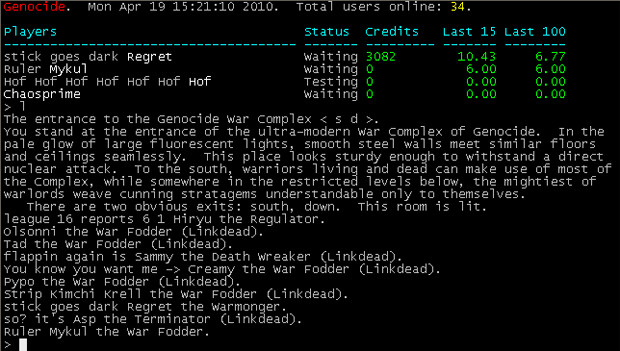
\includegraphics[width=0.8\textwidth]{images/mud_SS_2.jpg}
%  \caption[Captura de pantalla de juego MUD]{Captura de pantalla de MUD,
%  variante de Richard Bartle.}
%  \label{fig:MudClient}
%\end{figure}

El concepto básico fue inicialmente utilizado en la década de los ochenta con el
objetivo de mejorar y actualizar el juego llamado \emph{MUD}~\ref{fig:MudClient},
\emph{Multy User Dungeons}.

\section{Tipos de jugadores}

El desarrollador Richard Bartle, comenzó un análisis basado en los jugadores
donde encontró 4 estereotipos~\ref{fig:Players}.

\begin{itemize}
    \item {\bf Achievers:}
        Jugadores que se enfocan en obtener éxito mediante la obtención de puntos,
        premios, u otra forma de demostrar el trabajo puesto en el juego.
        Estos tipos de jugadores se esfuerzan la mayoría del tiempo en la obtención
        de dicho prestigio, lo que conlleva a casi una nula ventaja en la
        jugabilidad o avance en el juego.

    \item {\bf Explorers:}
        A estos jugadores les gusta explorar el mundo en el cual están inmersos,
        mas allá de lo geográfico, les interesan detalles dificiles de encontrar o
        caracteristicas escondidas del juego.
        La pasión detrás del conocer cada rincón del universo del juego los lleva
        a experimentar la mayor cantidad de casos y con esto logran conocer mejor
        el juego, mas alla de los propios desarrolladores.
        Un ejemplo de \emph{explorers} son jugadores solitarios, que buscan el
        poder descubrir lugares nuevos, aventurándose en el mundo del juego.

    \item {\bf Killers:}
        Este tipo de jugadores son los más competitivos, pues buscan destacarse
        dentro de los usuarios, creando drama entre otros jugadores.
        Algunos ejemplos de este tipo de jugadores son los \emph{Trolls},
        \emph{Hackers}, \emph{Cheaters}, etc.
        Pero no existen sólo aspectos negativos en éste tipo de jugadores,
        pues las personas que se dedican a un juego de forma profesional
        suelen apreciar la competitividad.

    \item {\bf Socializers:}
        Personas que son atraídas por la parte social de los juegos,
        en desmedro de la estrategia u otras partes de este.
        Se puede decir que estos jugadores son el ``Corazón'' del juego,
        pues ponen las relaciones interpersonales como la primera prioridad
        del juego en el que están inmersos.
        Los jugadores \emph{Socializers} consideran el juego
        como un vehículo para generar nuevas relaciones de amistad, y llevan
        sus grupos de juego, con los que comparten aventuras, al mundo real.

\end{itemize}

\begin{figure}[!htb]
  \centering
  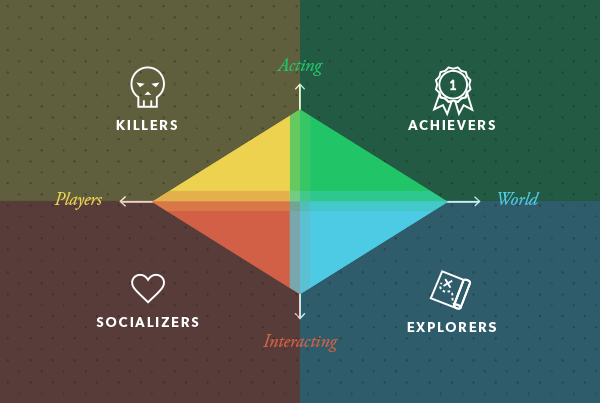
\includegraphics[width=0.8\textwidth]{images/TypeOfPlayersBartle.png}
  \caption[Tipos de esteriotipos de jugadores]{Tipos de jugadores por Richard Bartle}
  \label{fig:Players}
\end{figure}


Con esta información, el desarrollador modificó el juego para satisfacer cada
tipo de jugador.
Este cambio tuvo un gran éxito y demostró una nueva forma de atraer a diferentes
tipos de jugadores a un juego en particular, esto llamo la atención de empresas
que vieron este concepto como una nueva forma de atraer y retener a sus clientes.

\section{Definición}

Hoy en día {\GAM} se ha convertido en una herramienta para las empresas
para poder captar mas clientes.
Cada día aumenta el uso de este concepto por lo que es necesario entregar una
definición apropiada para el concepto.
{\GAM} se puede definir como ``el uso de elementos del diseño de juego en contextos
diferentes al de entretención''.
Para entender mejor los conceptos bajo esta definición se explicaran por partes:

\begin{itemize}
    \item {\bf Juego:}
        En primer lugar este concepto se refiere al juego en su totalidad,
        y no a la acción de jugar.
        Este concepto es caracterizado por un conjunto de reglas explícitas,
        que crean un ambiente en donde los jugadores buscan la competición para
        completar objetivos y metas.

    \item {\bf Elementos del diseño de juego}:
        Dentro de este concepto se puede encontrar 2 definiciones.
        La primera, es una definición estricta que sólo acepta ciertos elementos
        únicos.
        La segunda, es una definición en donde todos los elementos pueden ser
        utilizados.
        Para llegar a una definición robusta es necesario juntar ambas y así
        obtener un conjunto mas restrictivo en donde los elementos a utilizar
        son característicos a los juegos, que se encuentran en la mayoría de estos
        y que cumplen una rol importante en la jugabilidad de estos.

    \item {\bf Contextos diferentes al de juego:}
        Este es el concepto mas complejo de explicar debido a que es una idea
        abstracta.
        Una forma de explicarla es como una situación de la vida cotidiana
        que existe fuera de un juego o de un ambiente que contiene {\GAM}.

\end{itemize}

\section{Utilización}

Esta técnica a sido utilizada en diferentes áreas y contextos en todo el mundo,
del cual el Marketing ha sido una de las áreas más beneficiada con su
implementación.
Mas de 70 empresas en el ranking de \emph{Forbes Global $2000$} han utilizado o
piensan hacerlo con el motivo de una nueva fuente de marketing y como retención
de clientes\cite{Gam:Util:1}.
Un ejemplo exitoso del uso en marketing es \emph{Nike} con su aplicación
\emph{Nike+ Fuelband} que fue fue lanzada en enero del 2012\cite{Gam:Util:2}.
Con esta aplicación se logró crear un sistema gamificado en el cual se ayudaba
a sus clientes a mantener su estado física.
Otra empresa multinacional que a utilizado {\GAM} en marketing es \emph{McDonals}
con el uso de mecánicas de juego derivadas del juego de mesa \emph{Monopoly}.
Esta idea viene se viene implementando desde $1987$, por lo que al año $2010$
\emph{Mcdonals} incrementó sus ventas en los Estados Unidos en $5.6\%$
\cite{Gam:Util:2}.

{\GAM} también es utilizado como una herramienta para atraer y retener clientes,
adicionalmente es utilizado para alentar el correcto uso de un sitio web,
donde sitios web como StackOverflow y Samsung se aseguran de un sistema
de ranking por cada usuario y así establecer cierta fidelidad en respuestas
o reseñas.
StackOverflow, es una web dedicada a preguntas y respuestas sobre tecnología,
la cual entrega puntos  y logros a los usuarios al hacer determinadas tareas
de forma correcta.
Existen diferentes tipos de medallas y a medida  de que el usuario va ganando
puntos y reputación va obteniendo privilegios, siendo el mayor de estos ayudar a
moderar el sitio.
Samsung por su parte, también utiliza puntos y logros en su web pero esta
es enfocada a que los usuarios tengan interacción con la comunidad a nivel de
reseñas de productos y así crear contenido para la empresa\cite{Gam:Util:3}.

Educación y entrenamiento han sido otras áreas en donde a existido interés por
utilizar {\GAM}.
En los Estados Unidos, el departamento de educación de la ciudad de Nueva York
con el apoyo de \emph{MacArthur Foundation} y \emph{Bill and Melinda Gates
Foundation} crearon una escuela  llamada \emph{Quest to Learn}.
Lo que busca la escuela, es la modificación del sistema de aprendizaje,
utilizando mecanismos de juegos para así presentar la etapa de aprender
como algo mucho más llamativo para niños modernos\cite{Gam:Util:4}.

Otro sitio de educación utilizando esta técnica es \emph{Coursera},
compañía que se apoya de universidades de todo el mundo para enseñar
cursos sobre nuevos temas y tecnologías de manera gratuita vía e-learning.
La utilización de {\GAM} se ve reflejada en las medallas y certificados dados
a los estudiante, a medida que van completando tareas dentro del curso
hasta finalizarlo.
Dentro de todos los cursos dictados el mas popular es el de {\GAM}\cite{Gam:Util:5}.
En el año 2014, se inicio un proyecto llamado \emph{the True Life Game project}
que tiene como objetivo investigar las mejores formas de aplicar esta técnica en
la vida cotidiana.

Esta técnica también se usa en muchos otros ámbitos, pero en menor cantidad,
como productividad, autenticación, servicios financieros, entre otros.

\subsection{Empresas}

Diversas compañías actualmente usan {\GAM}, varias han creado plataformas para
aplicar sus principios y estrategias.
En $2007$, la compañía \emph{Bunchball}~\footnote{www.bunchball.com} fue una de
las primeras en implementar y proveer una plataforma gamificada como un
servicio\cite{Gam:Bunchball:1}.
\emph{Bunchball} tuvo clientes de gran tamaño como Bravo~\footnote{www.bravotv.com}
y \emph{The USA network}~\footnote{www.usanetwork.com}~\cite{Gam:Bunchball:2},
lo que significó el éxito del modelo adaptado para su plataforma web.

Otras grandes empresas que utilizan {\GAM} en la actualidad son:
SAP AG, IBM, EMC, CA, Slalom Consulting, Deloitte, Microsoft, LiveOps,
RedCritter~\cite{Gam:Companies:1}, etc.

Debido al peso que {\GAM} fue tomando dentro del mundo,
se crearon eventos para discutir sobre experiencias de éxito e ideas para
el futuro, como lo fue \emph{Gamification 2013},
un evento de discusión sobre su futuro~\cite{Gam:Events:1}.
En $2014$ se llevará a cabo \emph{Loyalty Gamification World Championship}
en San Francisco, USA~\cite{Gam:Events:2}.

\section{Críticas}

La idea de {\GAM}, desde sus inicios, a creado expectativas altas en todo el mundo
ya que ha sido utilizada por varias compañías, desde micro o pequeñas empresas
hasta multinacionales.
Pero existen retractores a la utilización de esta idea en la vida cotidiana.
Sebastian Detering, investigador de la universidad de Hamburgo, ha dicho que las
características mas utilizadas no son divertidas y crean una sensación falsa de
logro~\cite{Gam:Crit:1}.
A esto se a sumado personas relacionadas con el diseño de juegos como son
Jon Radoff y Margaret Robertson,  que declaran que la utilización de {\GAM}
excluye otras partes del diseño como son la historia, las experiencias de juego
y que lo utilizado en este concepto es de lo mas básico, faltando mecánicas de
juego~\cite{Gam:Crit:2}.

En el año 2012, la empresa analista \emph{Gartner} entregó un
reporte~\cite{Gam:Crit:3} en el cual explicaba que la idea de {\GAM}
"basaba su éxito en la nobleza del usuario y de las altas expectativas
de las empresas por utilizar esta idea".
También se esperaba de que para el año 2014 el 80\% de las aplicaciones
gamificadas fallarían debido a una falta de buen diseño,
esto producido por la falta de seriedad al crear las aplicaciones,
así como, el intento de copiar e implementar esto a la mayoría de las ideas.

{\GAM} ha experimentado un crecimiento exponencial en utilizacion durante los ultimos 
años. Ha sido utilizado en diversos contextos siendo el de ventas uno de los mas beneficiados
 y es por esto que la presente investigacion lo utilizara.
